%% This is file `elsarticle-template-1-num.tex',
%%
%% Copyright 2009 Elsevier Ltd
%%
%% This file is part of the 'Elsarticle Bundle'.
%% ---------------------------------------------
%%
%% It may be distributed under the conditions of the LaTeX Project Public
%% License, either version 1.2 of this license or (at your option) any
%% later version.  The latest version of this license is in
%%    http://www.latex-project.org/lppl.txt
%% and version 1.2 or later is part of all distributions of LaTeX
%% version 1999/12/01 or later.
%%
%% The list of all files belonging to the 'Elsarticle Bundle' is
%% given in the file `manifest.txt'.
%%
%% Template article for Elsevier's document class `elsarticle'
%% with numbered style bibliographic references
%%
%% $Id: elsarticle-template-1-num.tex 149 2009-10-08 05:01:15Z rishi $
%% $URL: http://lenova.river-valley.com/svn/elsbst/trunk/elsarticle-template-1-num.tex $
%%
% \documentclass[preprint,12pt]{elsarticle}
\documentclass[12pt]{elsarticle}

%% Use the option review to obtain double line spacing
%% \documentclass[preprint,review,12pt]{elsarticle}

%% Use the options 1p,twocolumn; 3p; 3p,twocolumn; 5p; or 5p,twocolumn
%% for a journal layout:
%% \documentclass[final,1p,times]{elsarticle}
%% \documentclass[final,1p,times,twocolumn]{elsarticle}
%% \documentclass[final,3p,times]{elsarticle}
%% \documentclass[final,3p,times,twocolumn]{elsarticle}
%% \documentclass[final,5p,times]{elsarticle}
%% \documentclass[final,5p,times,twocolumn]{elsarticle}

%% if you use PostScript figures in your article
%% use the graphics package for simple commands
%% \usepackage{graphics}
%% or use the graphicx package for more complicated commands
%% \usepackage{graphicx}
%% or use the epsfig package if you prefer to use the old commands
%% \usepackage{epsfig}

%% The amssymb package provides various useful mathematical symbols
\usepackage{amssymb}
%% The amsthm package provides extended theorem environments
%% \usepackage{amsthm}

%% The lineno packages adds line numbers. Start line numbering with
%% \begin{linenumbers}, end it with \end{linenumbers}. Or switch it on
%% for the whole article with \linenumbers after \end{frontmatter}.
% \usepackage{lineno}

%% natbib.sty is loaded by default. However, natbib options can be
%% provided with \biboptions{...} command. Following options are
%% valid:

%%   round  -  round parentheses are used (default)
%%   square -  square brackets are used   [option]
%%   curly  -  curly braces are used      {option}
%%   angle  -  angle brackets are used    <option>
%%   semicolon  -  multiple citations separated by semi-colon
%%   colon  - same as semicolon, an earlier confusion
%%   comma  -  separated by comma
%%   numbers-  selects numerical citations
%%   super  -  numerical citations as superscripts
%%   sort   -  sorts multiple citations according to order in ref. list
%%   sort&compress   -  like sort, but also compresses numerical citations
%%   compress - compresses without sorting
%%
%% \biboptions{comma,round}

% \biboptions{}


%\journal{}

\begin{document}

\begin{frontmatter}

%% Title, authors and addresses

%% use the tnoteref command within \title for footnotes;
%% use the tnotetext command for the associated footnote;
%% use the fnref command within \author or \address for footnotes;
%% use the fntext command for the associated footnote;
%% use the corref command within \author for corresponding author footnotes;
%% use the cortext command for the associated footnote;
%% use the ead command for the email address,
%% and the form \ead[url] for the home page:
%%
%% \title{Title\tnoteref{label1}}
%% \tnotetext[label1]{}
%% \author{Name\corref{cor1}\fnref{label2}}
%% \ead{email address}
%% \ead[url]{home page}
%% \fntext[label2]{}
%% \cortext[cor1]{}
%% \address{Address\fnref{label3}}
%% \fntext[label3]{}

    \title{Estudo de caso Monte Carlo cinético: \textit{High Current Density Eletrical Breakdown of $TiS_3$}}

%% use optional labels to link authors explicitly to addresses:
%% \author[label1,label2]{<author name>}
%% \address[label1]{<address>}
%% \address[label2]{<address>}

\author{Filipe Gonçalves Jacinto}

\address{Vitória, Espírito Santo}

\begin{abstract}
%% Text of abstract
Suspendisse potenti. Suspendisse quis sem elit, et mattis nisl. Phasellus consequat erat eu velit rhoncus non pharetra neque auctor. Phasellus eu lacus quam. Ut ipsum dolor, euismod aliquam congue sed, lobortis et orci. Mauris eget velit id arcu ultricies auctor in eget dolor. Pellentesque suscipit adipiscing sem, imperdiet laoreet dolor elementum ut. Mauris condimentum est sed velit lacinia placerat. Vestibulum ante ipsum primis in faucibus orci luctus et ultrices posuere cubilia Curae; Nullam diam metus, pharetra vitae euismod sed, placerat ultrices eros. Aliquam tincidunt dapibus venenatis. In interdum tellus nec justo accumsan aliquam. Nulla sit amet massa augue.
\end{abstract}

\begin{keyword}
Science \sep Publication \sep Complicated
%% keywords here, in the form: keyword \sep keyword

%% MSC codes here, in the form: \MSC code \sep code
%% or \MSC[2008] code \sep code (2000 is the default)

\end{keyword}

\end{frontmatter}

%%
%% Start line numbering here if you want
%%
%% \iinenumbers

%% main text
\section{Introdução}
\label{S:1}
Desde a síntese do Grafeno \cite{geim2010rise} materiais bidimensionais(2D) vem se mos- \linebreak trando como promissores candidatos para substituir os semicondutores convencionais baseados em Silício à medida em que se reduz a escala de dispositivos eletrônicos. Nesse sentido, são necessárias investigações mais profundas de materiais como o do $TiS_3$ (Trissulfeto de Titânio) que possuem algumas características como um  \textit{Gap} de $1~eV$ e pode ser isolado em monocamadas e nanotubos \cite{molina2017high}. 

O artigo indicado pelo professor da disciplina de Física computacional \cite{molina2017high} discute as propriedades de decomposição elétrica do $TiS_3$ onde os resultados que foram obtidos de forma experimental e através de simulações computacionais sugerem que este fenômeno ocorre tanto devido a efeito Joule quanto por dessorção de moléculas de $SO$ da superfície de $TiS_3$ em uma atmosfera rica em $O_2$ o que provoca a degradação do material e a consequente decomposição elétrica do $TiS_3$ .  

No contexto da disciplina de Física Computacional, este trabalho visa entender a dinâmica de dessorção de partículas no problema físico da decomposição elétrica do $TiS_3$ em condições ambientais utilizando a linguagem Python e o Método de Monte Carlo Cinético (KMC) discutindo os resultados obtidos e comparando-os com o do artigo em questão\cite{molina2017high}. Além disso, deve ser também um manual básico do uso do código desenvolvido.Para isso, pretende-se utilizar alguns resultados ja disponibilizados pelo professor como as energias de formação de vacâncias calculadas utilizando o pacote Quantum Espresso\cite{giannozzi2009quantum} , e a termogravimetria disponibilizada no artigo\cite{molina2017high} para calcular a dinâmica de dessorção do $S$ da monocamada de $TiS_3$ rica em$ O_2$ e compara-la com o experimento.

% \begin{itemize}
% \item Bullet point one
% \item Bullet point two
% \end{itemize}
% 
% \begin{enumerate}
% \item Numbered list item one
% \item Numbered list item two
% \end{enumerate}

\section{Metodologia} Para estudar a dinâmica de dessorção do $S$ da monocamada de $TiS_3$ foram contruídos códigos em python utilizando a estrutura de algoritmo KMC em específico o método Bortz-Kalos-Lebowitz (BKL) que é utilizado para estudar a evolução no tempo de um sistema onde os processos podem ser estudados através de uma taxa conhecida nesse caso $R_i$ e podem ser descritas ao longo do tempo através dos seguintes passos:
\begin{enumerate}
\item Fixar o o tempo inicial t = 0;
\item Criar uma lista com todas a probabilidades $\Delta_i$ do sistema;
    
    Este passo é extremamente importante, pois aqui esta uma parte da Física do sistema , os eventos $\Delta_i$ são as energias associadas a cada evento de dessorção descrito nas Tabelas~\ref{t1} e~\ref{t2}. Através de cada $\Delta_i$ pode-se calcular as probabilidades de ocorrência de cada evento ($\Gamma_i$) através da equação~\ref{eq1} onde $\Gamma_{i}^{0}= 10^{13}~s^{-1}$ e é a frequência de ocorrência de cada evento.
\begin{table}[ht]
\centering
\begin{tabular}{| l| l| l| l|}
\hline
\textbf{Evento} & \textbf{Sistema} & \textbf{Defeito} & \textbf{Energia (\textit{eV})}\\
\hline  
\hline
1 & $TiS_3O_{0.50}$ & Defeito de $SO$ (primeiro)   & 1.23 \\
\hline
2 & $TiS_3O_{0.50}$ & Defeito de $SO$ + monovacância & 1.55 \\
\hline
3 & $TiS_3O_{0.50}$ & Defeito de $SO$ + monovacância& 1.63 \\
\hline
4 & $TiS_3O_{0.50}$ &  Defeito de $SO$ (divacância)& 2.61 \\
\hline
\end{tabular}
\caption{Tabela com a respectiva energia de ativação de cada evento para uma superfície com $50\%$ de Oxigênio.}
\label{t1}
\end{table}

\begin{table}[ht]
\centering
\begin{tabular}{| l| l| l| l|}
\hline
\textbf{Evento} & \textbf{Sistema} & \textbf{Defeito} & \textbf{Energia (\textit{eV})}\\
\hline  
\hline
1 & $TiS_3O_{0.25}$ & Defeito de $SO$ (primeiro)   & 1.23 \\
\hline
2 & $TiS_3O_{0.25}$ & Defeito de $SO$ + monovacância & 1.51 \\
\hline
3 & $TiS_3O_{0.25}$ & Defeito de $SO$ + monovacância& 1.78 \\
\hline
4 & $TiS_3O_{0.25}$ &  Defeito de $SO$ (divacância)& 2.62 \\
\hline
\end{tabular}
\caption{Tabela com a respectiva energia de ativação de cada evento para uma superfície com $25\%$ de Oxigênio.}
\label{t2}
\end{table}



    \begin{equation}
        \Gamma_i = \Gamma_{i}^{0}\exp{\left({\frac{-\Delta_i}{K_b T}}\right)}
        \label{eq1}
    \end{equation}

\item Calcular a função acumulativa $R_n$ que é a soma da probabilidade acumulativa dos eventos que pode ser feita de acordo com a Equação~\ref{eq2} onde $R_i$ é a probabilidade de cada evento , $N_i$ número de partículas que podem realizar o i-ésimo evento e $n_e$ o número total de eventos considerados possíveis; 

    \begin{equation}
        R_n = \sum_{i=1}^{n_e} R_i = \sum_{i=1}^{n_e} \Gamma_i N_i
        \label{eq2}
    \end{equation}

\item Gerar um número aleatório em relação a uma distribuição uniforme entre $u \in~(0,1]$;
\item Encontrar qual será a transição que ocorerá , ou seja, verificar qual termo da lista de probabilidade $R_i$ que respeita a condição da inequação~\ref{eq3}: 
    \begin{equation} 
    R_{i-1} < uR_n < R_i
    \label{eq3}
    \end{equation}

\item Realizar a transição. Este passo depende muito do sistema em questão, nesse caso em específico fazer a transição significa levar em conta a mudança na lista de partículas dos eventos possíveis, além disso para calcular a massa perdida leva-se em conta que um evento para uma monovacância isto é o número de átomos diminui em um único átomo, já para o um divacância o número total de partículas será reduzido em dois.

\item Gerar um novo número aleatório em relação a uma distribuição uniforme entre $u \in~(0,1]$;
\item Realizar uma translação temporal $t \rightarrow t+\Delta t$ onde $\Delta t$ é dada pela equação~\ref{eq4}:
    \begin{equation}
        \Delta t = R^{-1} \ln{(1/u)}
        \label{eq4}
    \end{equation}

\item Atualizar a os valores de $R_i$ a partir das transição realizada e recalcular o valor de $R_n$; 
\item Voltar ao passo 2.

\end{enumerate}




\section{Resultados e Discussão} 

\begin{figure}[!htbp]
%\centering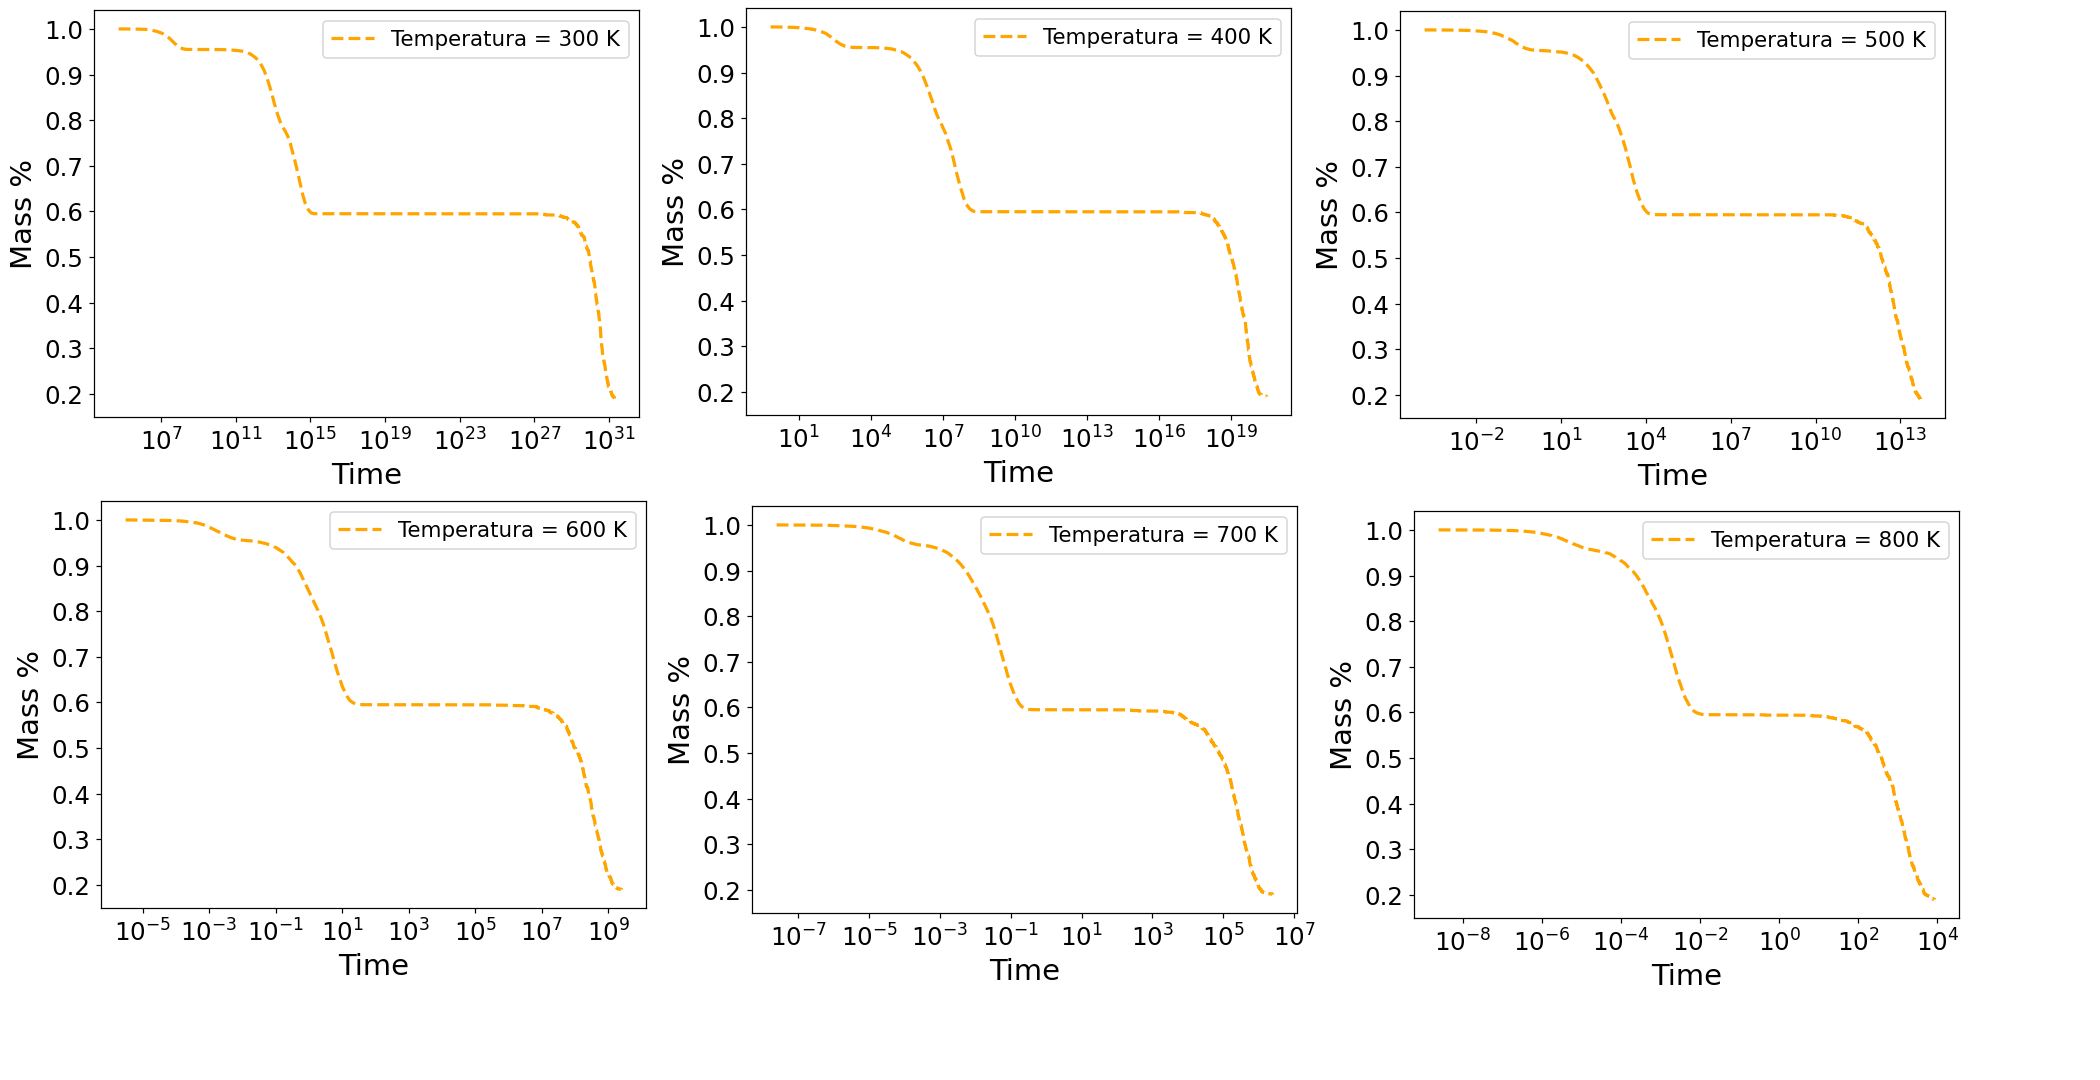
\includegraphics[width=1\linewidth]{figures/var-massa-tempo.png}
\centering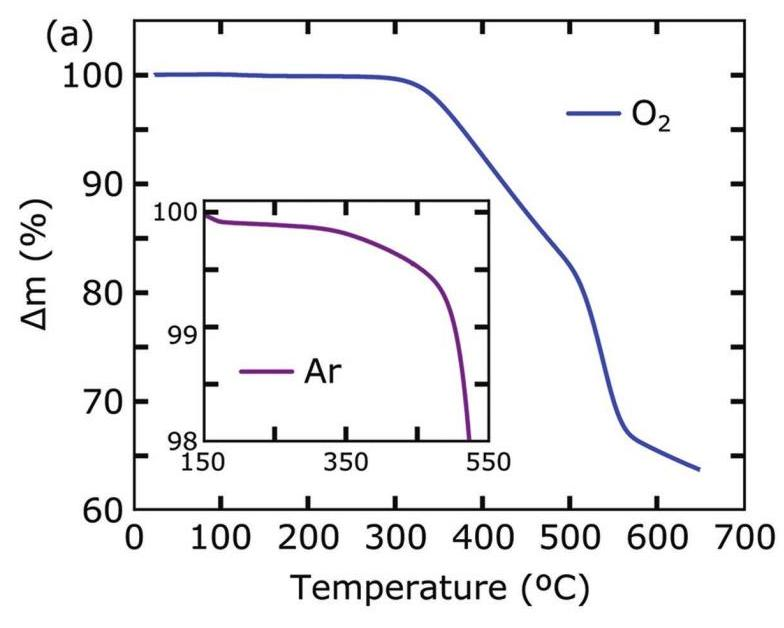
\includegraphics[scale=0.35]{figures/var-massa-temp.jpg}
\caption{Curva de termogravimetria para o \texit{bulk} de $TiS_3$ .}
\label{f1}
\end{figure}
De forma a estudar o papel da perda de massa do $TiS_3$ no fenômeno de decomposição elétrica foram analisados resultados de alguns experimentos sendo um desses o de termogravimetria. A Figura \ref{f1} apresenta a curva de termogravimetria sob efeito de uma atmosfera rica em $O_2$ obtida experimental- \linebreak mente\cite{molina2017high}. Observando a Figura \ref{f1} pode-se ver uma variação de massa de $36\%$ em um intervalo de temperatura de $27~^\circ C$ até $650~^\circ C$. Nesse intervalo de temperatura pode-se notar dois eventos a citar: (1) no intervalo de  $300-400~^\circ C$ com uma variação de massa de $18\%$ e (2) no intervalo de $450-550~^\circ C$ com uma variação de massa também de $18\%$. 


\begin{figure}[!htbp]
%\centering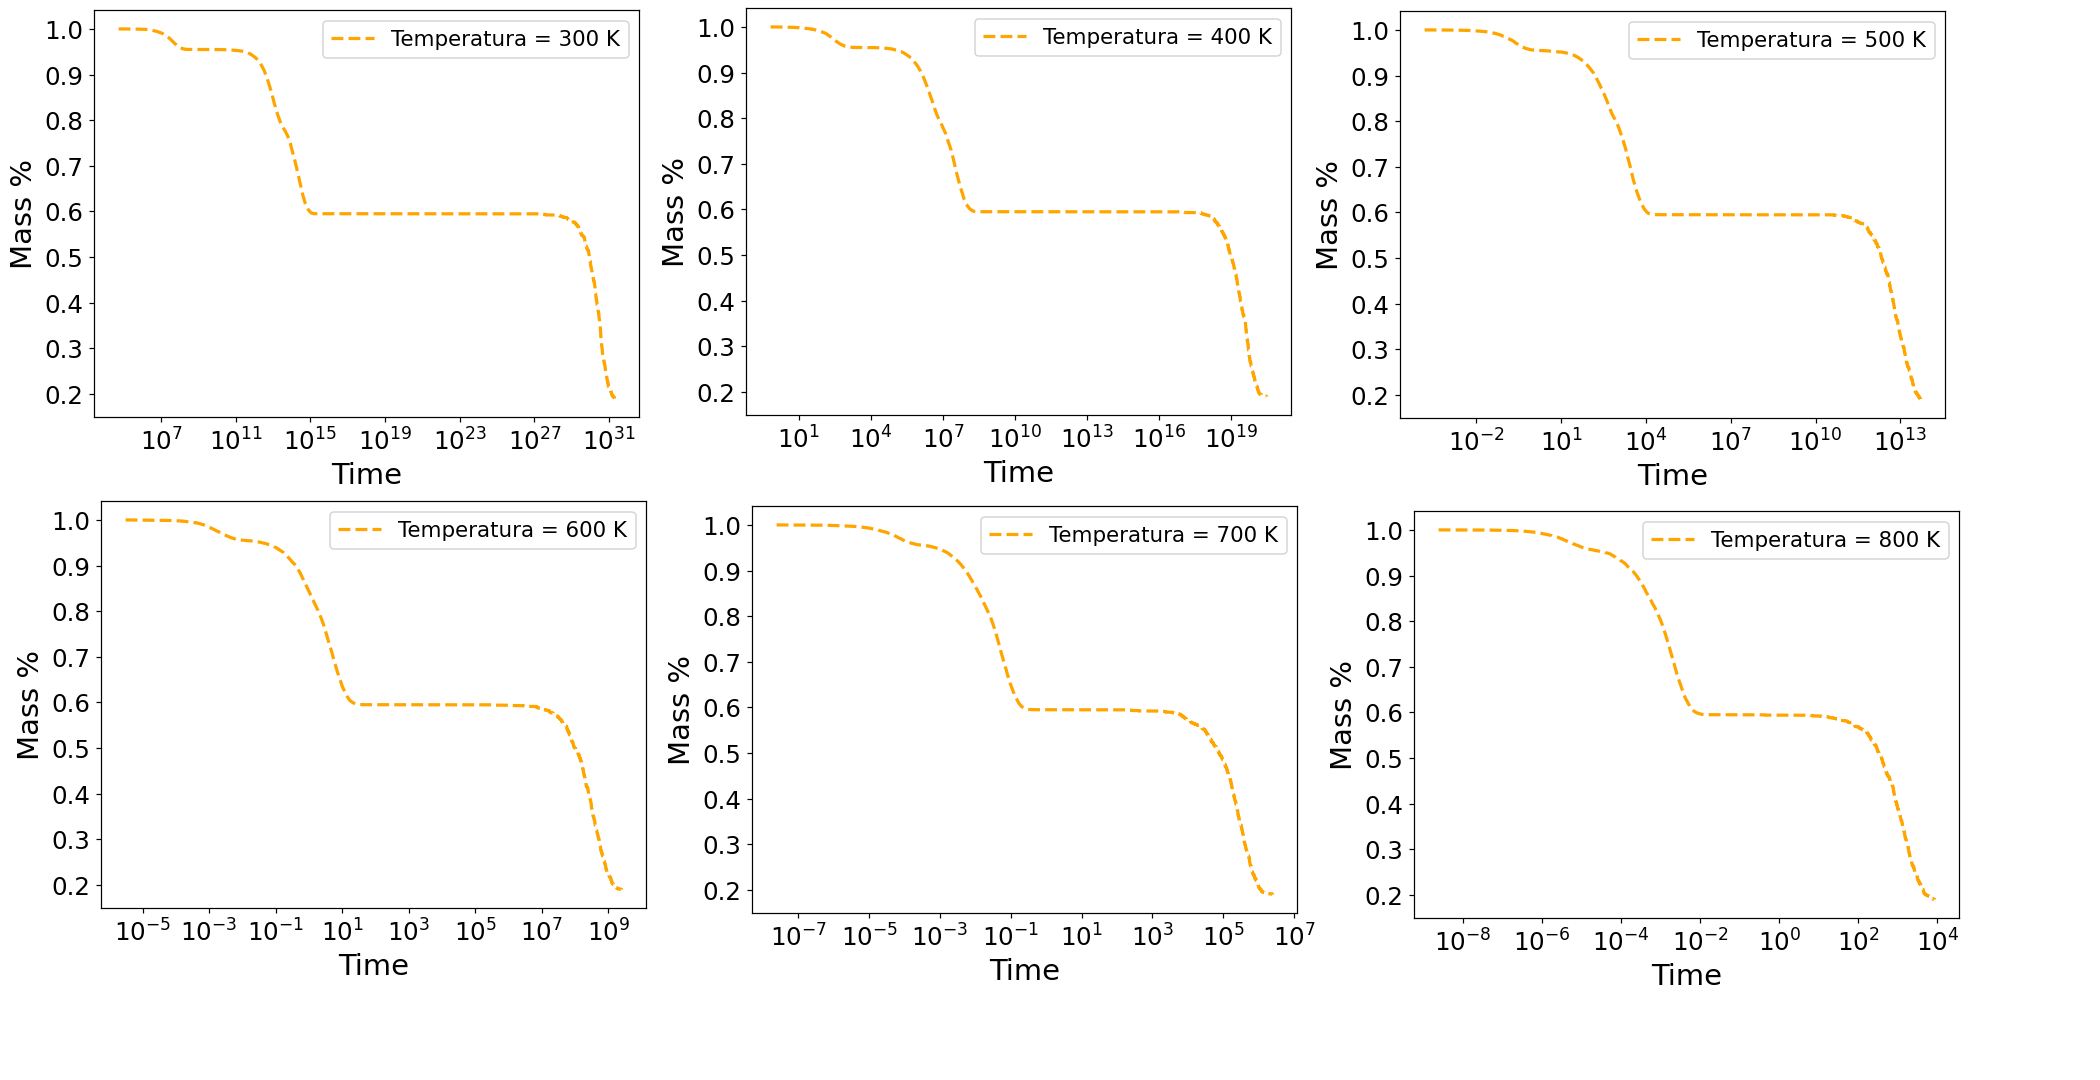
\includegraphics[width=1\linewidth]{figures/var-massa-tempo.png}
\centering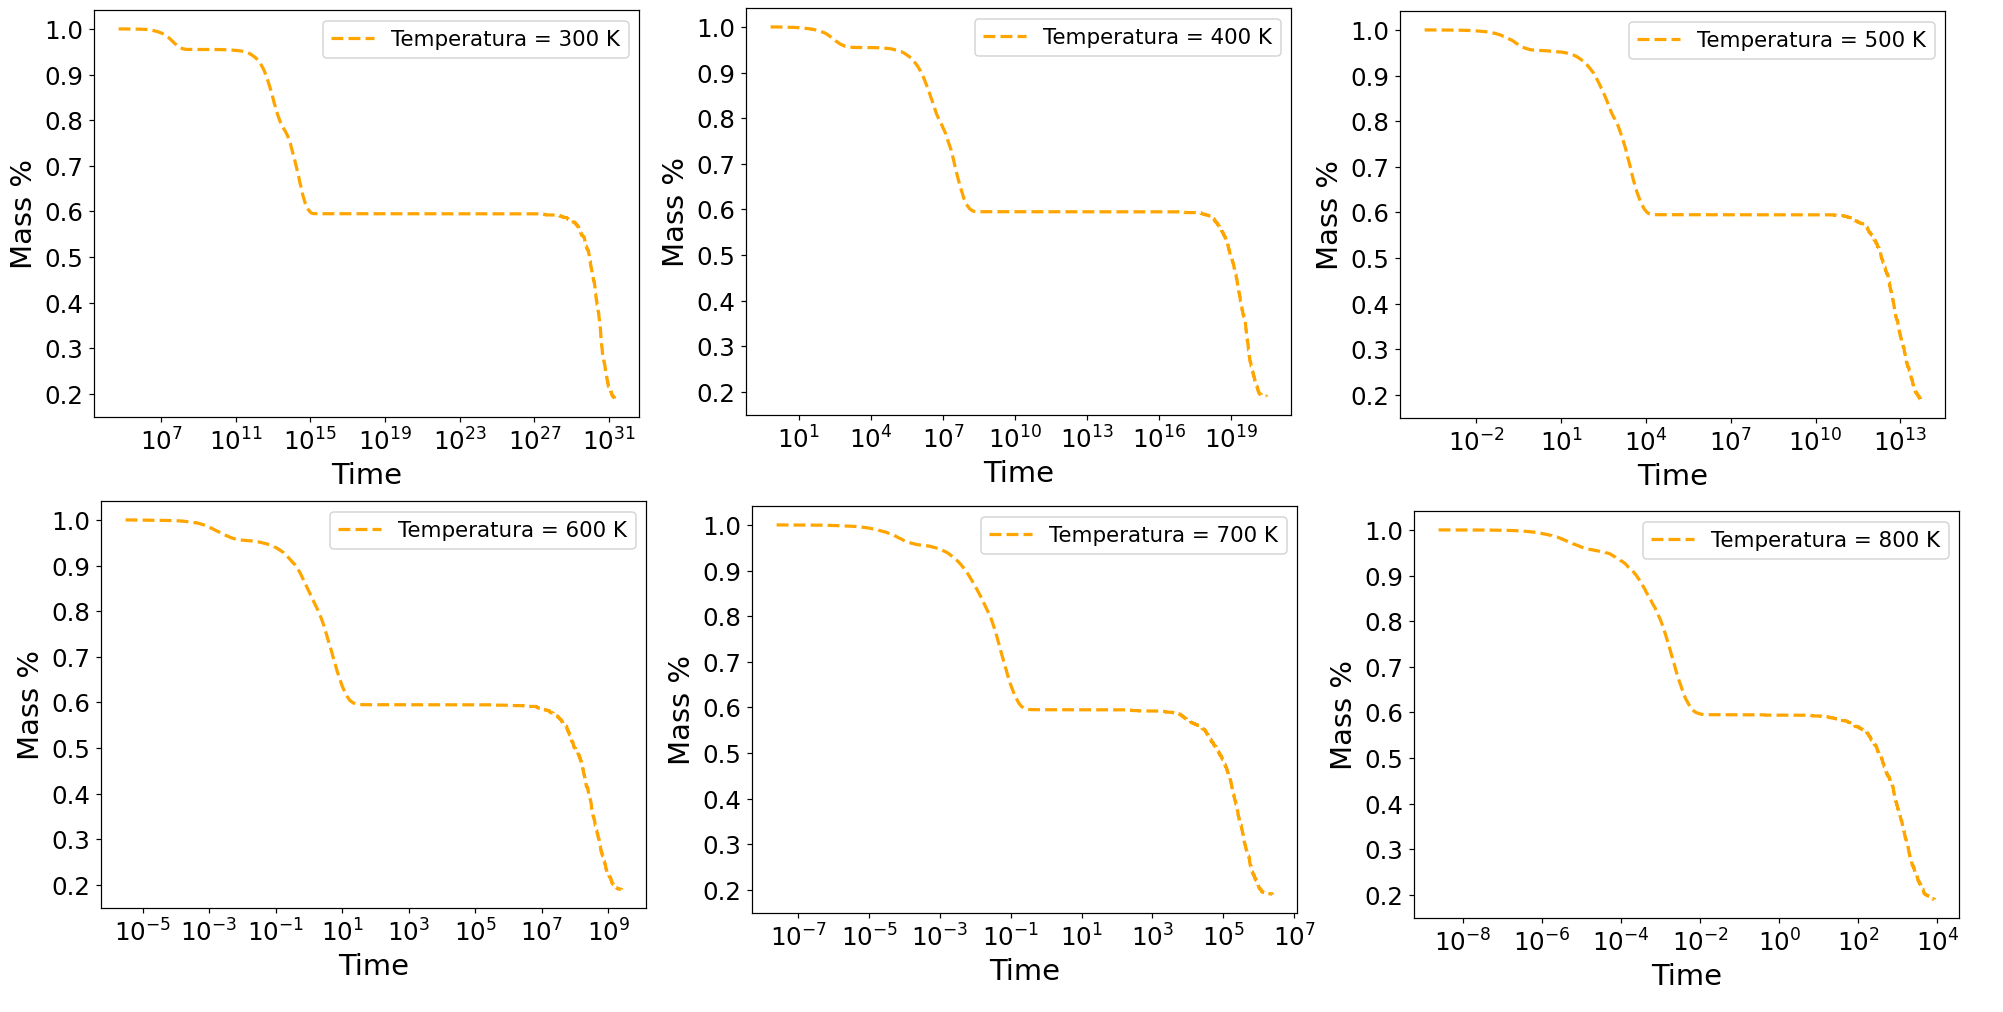
\includegraphics[scale=0.8]{figures/var-massa-tempo-2.png}
\caption{Curva da variação de massa em relação ao tempo obtida através do método de monte carlo cinético para uma superfície com $50\%$ de $0_2$ . }
\label{f2}
\end{figure}

\begin{figure}[!htbp]
%\centering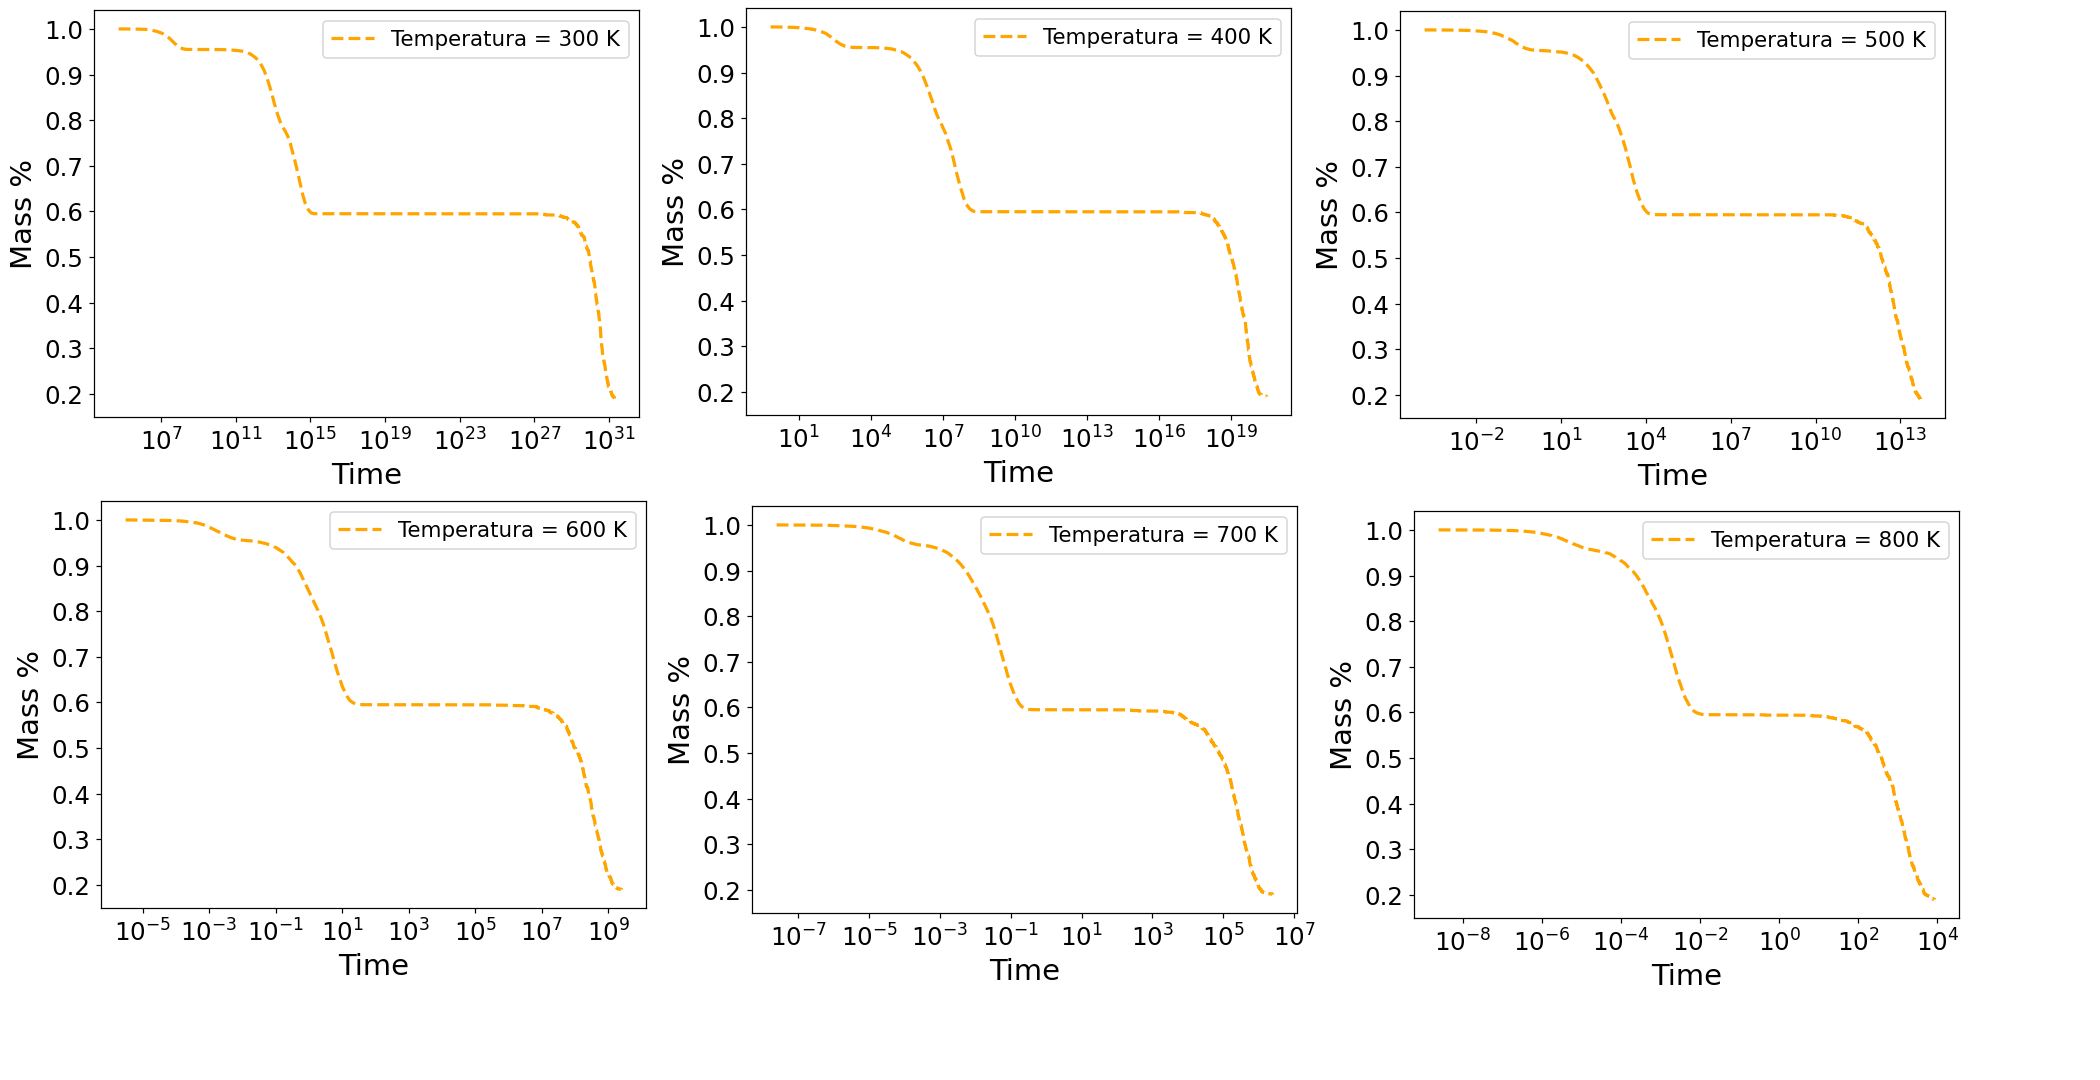
\includegraphics[width=1\linewidth]{figures/var-massa-tempo.png}
\centering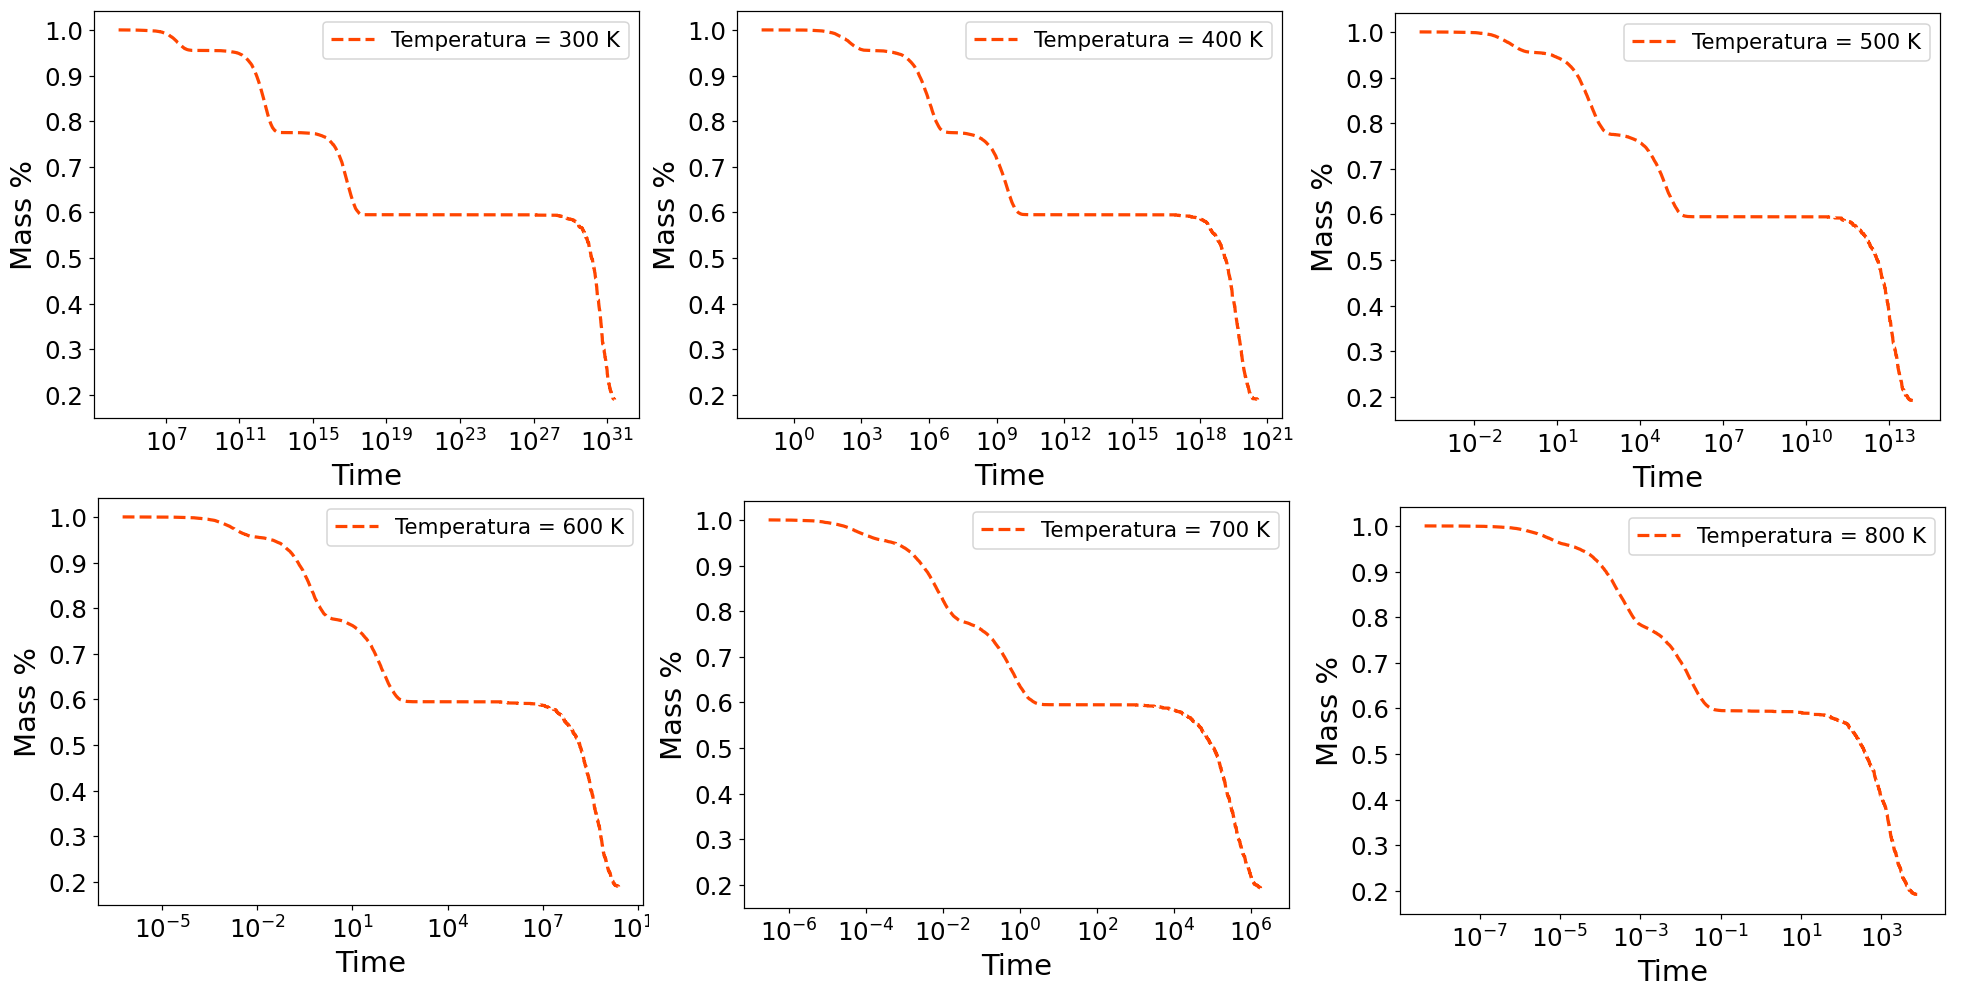
\includegraphics[scale=0.8]{figures/var-massa-tempo-25.png}
\caption{Curva da variação de massa em relação ao tempo obtida através do método de monte carlo cinético para uma superfície com $25\%$ de $0_2$ . }

\label{f3}
\end{figure}

De forma a investigar a dinâmica do sistema de dessorção de átomos de $S$ do $TiS_3$ foi aplicado o método de Monte Carlo cinético calculando primeiro a variação de massa em porcentagem ao longo do tempo mantida uma temperatura constante. Este resultado é apresentado nas Figuras~\ref{f2} e~\ref{f3} onde o modelo considera que o sistema é uma monocamda de $TiS_3$ exposta a uma Atmosfera com $50\%$ e $25\%$ de concentração de $O_2$ respectivamente. Pode-se ver pelas Figuras~\ref{f2} e~\ref{f3} que a perda de massa é mais rápida quanto maior for a temperatura considerada para os cálculos. 

Além disso, as energias de ativação de cada evento tem participação importante na dinâmica do sistema já que energias maiores terão uma probabilidade menor de acontecer e portanto em geral ocorrerão depois que os eventos de menor energia se tornarem menos prováveis devido a diminuição do número de partículas disponíveis para que estes ocorram. Este comportamento se torna claro quando se analisa a Figura~\ref{f3} onde a diferença de energia entre cada evento é maior e observa-se um número maior de degraus bem definidos no gráfico. Estes degraus denotam quando cada evento ocorre com maior frequência sendo que os de menor energia ocorrem sempre primeiro. 

\begin{figure}[!htbp]
%\centering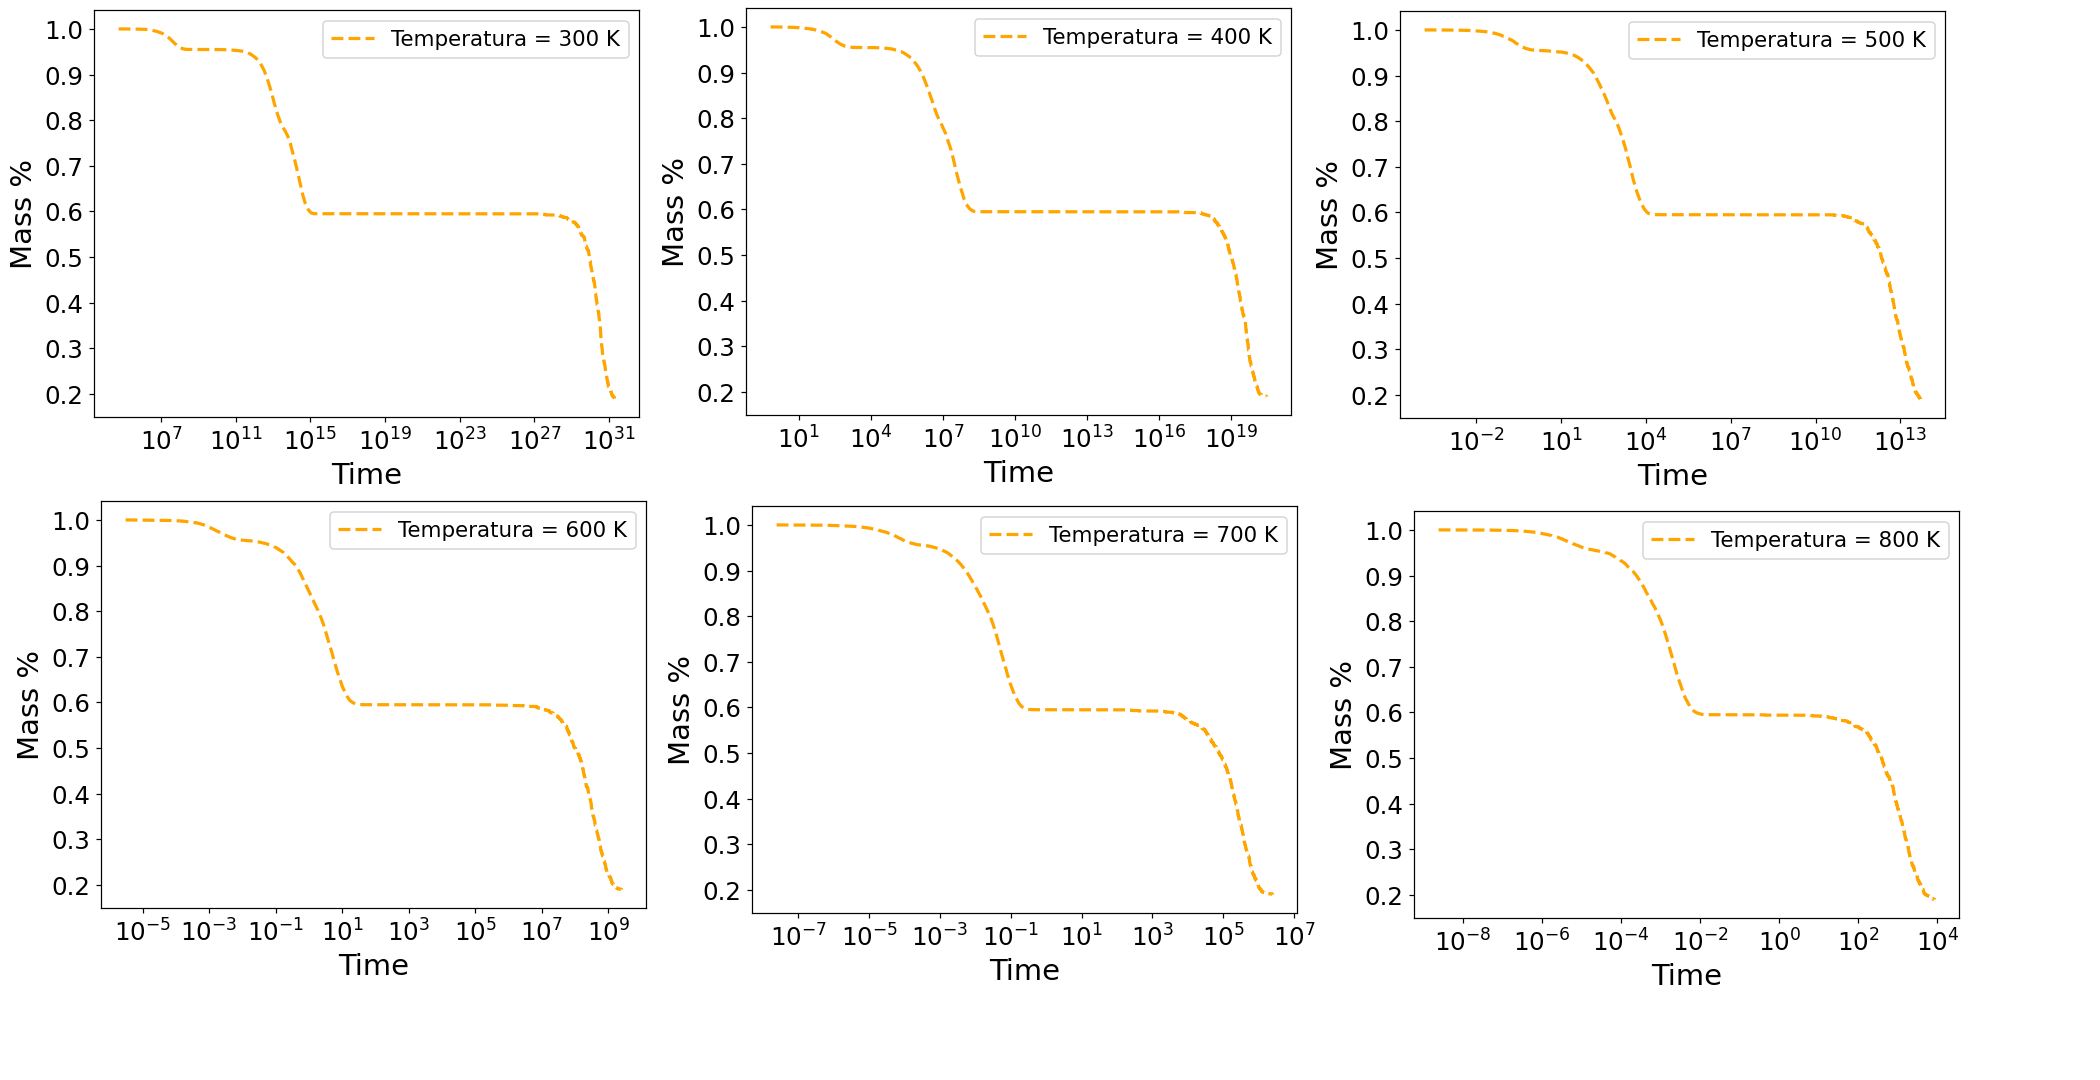
\includegraphics[width=1\linewidth]{figures/var-massa-tempo.png}
\centering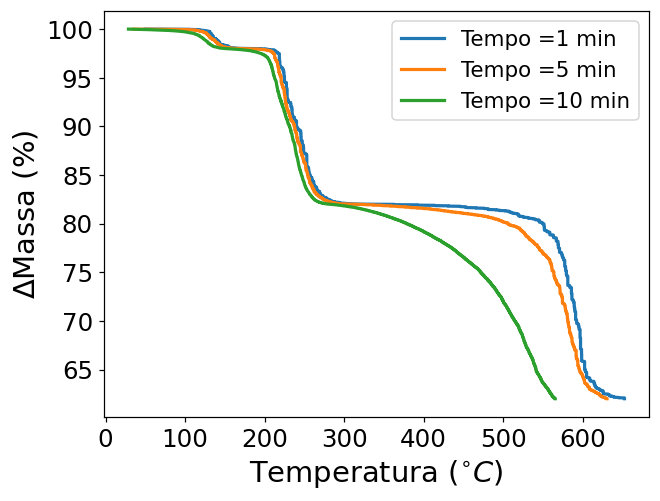
\includegraphics[scale=0.6]{figures/Temperatura-massa.png}
\caption{Curva da variação de massa em relação a temperatura para diferentes intervalos de tempo descritos na legenda, em uma superfície com $50\%$ de $O_2$.}
\label{f4}
\end{figure}


Finalmente, de forma a comparar os resultados obtidos na curva de termogravimetria apresentada na Figura \ref{f1}, o método de KMC foi utilizado variando a temperatura em escalas de tempo diferentes. Este resultado é apresentado na Figura \ref{f4}. Pode-se ver na Figura \ref{f4} assim como na Figua \ref{f1} à ocorrência de dois eventos embora em diferentes intervalos de temperatura. O evento (1) ocorre no intervalo de $150-250~^\circ C$ com uma variação de massa de $17.5\%$ que se deve principalmente por formações de monovacâncias e o evento (2) ocorre no intervalo de  $500-600~^\circ C$ com uma variação de massa de $21.5\%$ que por sua vez se deve principalmente a formação de divacâncias. 


%% The Appendices part is started with the command \appendix;
%% appendix sections are then done as normal sections
%% \appendix

%% \section{}
%% \label{}

%% References
%%
%% Following citation commands can be used in the body text:
%% Usage of \cite is as follows:
%%   \cite{key}          ==>>  [#]
%%   \cite[chap. 2]{key} ==>>  [#, chap. 2]
%%   \citet{key}         ==>>  Author [#]

%% References with bibTeX database:

\bibliographystyle{model1-num-names}
\bibliography{sample.bib}

%% Authors are advised to submit their bibtex database files. They are
%% requested to list a bibtex style file in the manuscript if they do
%% not want to use model1-num-names.bst.

%% References without bibTeX database:

% \begin{thebibliography}{00}

%% \bibitem must have the following form:
%%   \bibitem{key}...
%%

% \bibitem{}

% \end{thebibliography}


\end{document}

%%
%% End of file `elsarticle-template-1-num.tex'.
